\documentclass[a4paper,12pt]{article}

\usepackage{fancyhdr}
\usepackage{lastpage}
\usepackage{amsmath}
\usepackage{tikz}
\usepackage{amsfonts}
\pagestyle{fancy}
\lhead{Samuel Loomis}
\setlength{\headheight}{15pt}
\chead{Electromagnetism HW 1}
\rhead{\thepage\ of \pageref{LastPage}}
\lfoot{}
\cfoot{}
\rfoot{}

\begin{document}

\subsection*{Question 1}

\begin{picture}(300,200)

\linethickness{3pt}
\put(100,0){\line(0,1){200}}
\put(0,100){\line(1,0){390}}
\put(10,80){\line(1,0){30}}
\put(12.5,75){\line(1,0){25}}
\put(15,70){\line(1,0){20}}
\put(17.5,65){\line(1,0){15}}
\put(150,150){\circle*{4}}
\put(50,150){\circle{4}}
\put(50,50){\circle*{4}}
\put(150,50){\circle{4}}
\linethickness{1pt}
\put(150,125){\vector(0,1){20}}
\put(150,125){\vector(0,-1){20}}
\put(125,150){\vector(1,0){20}}
\put(125,150){\vector(-1,0){20}}
\put(150,75){\vector(0,1){20}}
\put(150,75){\vector(0,-1){20}}
\put(75,150){\vector(1,0){20}}
\put(75,150){\vector(-1,0){20}}
\put(50,125){\vector(0,1){20}}
\put(50,125){\vector(0,-1){20}}
\put(125,50){\vector(1,0){20}}
\put(125,50){\vector(-1,0){20}}
\put(50,75){\vector(0,1){20}}
\put(50,75){\vector(0,-1){20}}
\put(75,50){\vector(1,0){20}}
\put(75,50){\vector(-1,0){20}}
\put(25,65){\line(0,1){35}}
\put(155,155){$q$}
\put(122.5,155){$d_1$}
\put(155,122.5){$d_2$}
\put(67.5,155){$d'_1$}
\put(155,70){$d'_2$}
\put(40,155){$q'_1$}
\put(155,45){$q'_2$}
\put(40,40){$q''$}




\end{picture}
\\
The infitnite plates will have induced charges on them, each
independently will act like an imaginary charge $q'$ with the same charge but
opposite sign as $q$.  With both of the plates together, the induced
charges on one plate will effect the charge $q$ and also the imaginary
charges $q'_1$ and $q'_2$.  This interaction will be like having
another imaginary charge $q''$ in the lower left corner shown in the
modified diagram.  This charge should be equal and opposite to the
first imaginary charge, and thus $q'' = q$  Thus to calculate the
force exerted on $q$, a calculation can be done as if negative charges
$q'_1$\ and $q'_2$ as well as a positive charge $q''$ are placed in a
quadrapole configuration.

The force on $q$ is equal to the sum of the three forces:
$F_1$ from $q'_1$, $F_2$ from $q'_2$ and $F_3$
from $q''$.  Using equation (\ref{1}) and substituting the proper
charge in for Q, the three forces can be found.  Adding them together
will give the total force $\mathbf{F_T}$.
\begin{align}
\mathbf{F}&=\frac{1}{4\pi\epsilon_0}\frac{qQ}{r^2}\hat{r}\label{1}\\
\mathbf{F_1}&=\frac{1}{4\pi\epsilon_0}\frac{q(-q)}{(2d_1)^2}\hat{x}\\
\mathbf{F_2}&=\frac{1}{4\pi\epsilon_0}\frac{q(-q)}{(2d_2)^2}\hat{y}\\
\mathbf{F_3}&=\frac{1}{4\pi\epsilon_0}\frac{q(q)}{(2d_1)^2}\frac{\sqrt{2}}{2}\hat{x}+\frac{1}{4\pi\epsilon_0}\frac{q(q)}{(2d_2)^2}\frac{\sqrt{2}}{2}\hat{y}\\
\mathbf{F_T}&=\frac{\sqrt{2}-2}{32(d_1)^2\pi\epsilon_0}q^2\hat{x}+\frac{\sqrt{2}-2}{32(d_2)^2\pi\epsilon_0}q^2\hat{y}
\end{align}
\\
\textbf{Q.1 cont}\ I am guessing that the far field potential goes like a
$\frac{1}{r^3}$ at values of $r>>2d$, much like a quadrupole would behave.


\subsection*{Question 2}
\subsubsection*{(a)}
Prove the Green's reciprocity theorem:

\[
\int_{allspace}\rho_1\phi_2d^3r=\int_{allspace}\rho_2\phi_1d^3r
\]
Evaluating the integral $\int\mathbf{E_1}\cdot\mathbf{E_2}d^3r$
substituting $\mathbf{E_1}=-\vec\bigtriangledown\phi_1$ by parts:
\begin{align}
\int
-\vec\bigtriangledown\phi_1\cdot\mathbf{E_2}d^3r&=(-\phi_1\mathbf{E_2})\big|_{allspace}-\int-\phi_1\vec\bigtriangledown\cdot\mathbf{E_2}d^3r\\
\int
-\vec\bigtriangledown\phi_1\cdot\mathbf{E_2}d^3r&=
\frac{1}{\epsilon_0}\int\phi_1\rho_2d^3r
\end{align}Note that: $(-\phi_1\mathbf{E_2})\big|_{allspace}=0$.\\
Then evaluating the same integral substituting
$\mathbf{E_2}=-\vec\bigtriangledown\phi_2$\ again by parts:
\begin{align}
\int\mathbf{E_1}\cdot-\vec\bigtriangledown\phi_2d^3r&=(-\phi_2\mathbf{E_1})\big|_{allspace}-\int\phi_2\vec\bigtriangledown\cdot\mathbf{E_1}d^3r\\
\int\mathbf{E_1}\cdot-\vec\bigtriangledown\phi_2d^3r&=\frac{1}{\epsilon_0}\int\phi_2\rho_1d^3r
\end{align}
Thus:
\begin{align}
 \int\phi_1\rho_2d^3r=\int\phi_2\rho_1d^3r
\end{align}
\subsubsection*{(b)}

If putting a charge Q on A generates a potential $V_{AB}$ on B and
another $V_{AA}$ on A, wouldn't generating a charge Q on B generate
$V_{BA}$ on a AND $V_{BB}$ on B?  For the same reason?  Thus, wouldn't $V_{BB}+V_{BA}=V_{AB}+V_{AA}$?

\subsection*{Question 3}

The hemisphere is neutral to begin with, when placed in an electric
field $\mathbf{E_0}$ the hemisphere will polarize.  I am not sure if
the polarization will be as displayed here, or a more dificult
polarization with more negative charge twords the outer rim of the
flat surface of the sphere.

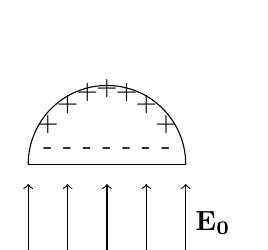
\begin{tikzpicture}
\draw (0,10) arc (0:180:1cm);
\draw (0,10) -- (-2,10);
\draw[->] (0   ,8.75) -- (0   ,9.75);
\draw[->] (-.5 ,8.75) -- (-.5 ,9.75);
\draw[->] (-1  ,8.75) -- (-1  ,9.75);
\draw[->] (-1.5,8.75) -- (-1.5,9.75);
\draw[->] (-2  ,8.75) -- (-2  ,9.75);
\draw (0,9.25) node[right] {$\mathbf{E_0}$};
\draw (-.5,10) node[above] {-};
\draw (-.25,10) node[above] {-};
\draw (-.75,10) node[above] {-};
\draw (-1,10) node[above] {-};
\draw (-1.25,10) node[above] {-};
\draw (-1.5,10) node[above] {-};
\draw (-1.75,10) node[above] {-};
\draw (-.25,10.75) node[below] {+};
\draw (-.5,11) node[below] {+};
\draw (-.75,11.15) node[below] {+};
\draw (-1,11.2) node[below] {+};
\draw (-1.25,11.15) node[below] {+};
\draw (-1.5,11) node[below] {+};
\draw (-1.75,10.75) node[below] {+};
\end{tikzpicture}

The boundary conditions of the hemisphere are $(i)V=0$ when $r=R$
and $0\le\theta\le\frac{\pi}{2}$, $(ii)V=0$ when $0\le r\le R$ and
$\theta=\frac{\pi}{2}$ and finally $(iii)V=-E_0r\ cos\ \theta+ C$ when
$r>>R$.  Unlinke the sphere
problem, I don't see an easy way to state that the potential is 0 for
an entire plane and thus C cannot be eliminated right away.

Starting with the phi angle symetric version of the spherical Laplace
equation:
\begin{align}
V(r,\theta)&=\sum\limits_{l=0}^\infty(A_lr^l+\frac{B_l}{r^{l+1}})P_l(cos\ \theta)
\end{align} Boundary conditions are used to solve for $A_l$ and $B_l$.
$P_l(cos\ \theta)$ is the Legandre polynomial for $cos\ \theta$.

From boundary condition $(i)$:
\begin{align}
0&=A_lR^l+\frac{B_l}{R^{l+1}}\  for\  0\le\theta\le\frac{\pi}{2}
\end{align}

 So in the northern hemisphere:
\begin{align}
B_l&=-A_lR^{2l+1}\\
V(r,\theta)&=\sum\limits_{l=0}^\infty
A_l(r^l-\frac{R^{2l+1}}{r^{l+1}})P_l(cos\ \theta)
\end{align}

From boundary condition $(iii)$ $r>>R$ the second term is very small
and thus:
\begin{align}
\sum\limits_{l=0}^\infty A_lr^lP_l(cos\ \theta)= -E_0r\ cos\ \theta+C
\end{align}Since the result has $cos\ \theta$ and C, only $l=0,\ l=1$
matter. $A_0=C$ and $A_1=-E_0$
\begin{align}
V(r,\theta)&=C\frac{R}{r}-E_0(r-\frac{R^3}{r^2})cos\ \theta
\end{align}\\
To eliminate C, I will simply drop it and test the boundary
conditions.  Does (\ref{potential}) satisfy my boundary conditions?
\\
\begin{align}
V(r,\theta)&=-E_0(r-\frac{R^3}{r^2})cos\ \theta\label{potential}\\
(i)\ r=R:\ \ 0&\overset{?}{=}-E_0(R-\frac{R^3}{R^2})cos\ \theta\\
0&\overset{\checkmark}{=}R-R\\
(ii)\ \theta=\frac{\pi}{2}:\ \ 0&\overset{?}{=}-E_0(r-\frac{R^3}{r^2})cos\ \frac{\pi}{2}\\
0&\overset{\checkmark}{=}cos\ \frac{\pi}{2}\\
(iii)\ r>>R:\ \ V(r,\theta)&\overset{\checkmark}{\rightarrow}-E_0r\ cos\ \theta: C=0
\end{align}
The conductor will look like a dipole far away.
\end{document}


